
\documentclass[11pt,a4paper]{article}
\usepackage[utf8]{inputenc}
\usepackage[margin=1in]{geometry}
\usepackage{graphicx}
\usepackage{booktabs}
\usepackage{hyperref}
\usepackage{listings}
\usepackage{xcolor}
\usepackage{authblk}
\usepackage{pgfplots}
\pgfplotsset{width=10cm,compat=1.9}

\definecolor{codegreen}{rgb}{0,0.6,0}
\definecolor{codegray}{rgb}{0.5,0.5,0.5}
\definecolor{codepurple}{rgb}{0.58,0,0.82}
\definecolor{backcolour}{rgb}{0.95,0.95,0.92}

\lstdefinestyle{mystyle}{
    backgroundcolor=\color{backcolour},   
    commentstyle=\color{codegreen},
    keywordstyle=\color{magenta},
    numberstyle=\tiny\color{codegray},
    stringstyle=\color{codepurple},
    basicstyle=\ttfamily\footnotesize,
    breakatwhitespace=false,         
    breaklines=true,                 
    captionpos=b,                    
    keepspaces=true,                 
    numbers=left,                    
    numbersep=5pt,                  
    showspaces=false,                
    showstringspaces=false,
    showtabs=false,                  
    tabsize=2
}

\lstset{style=mystyle}

\title{\textbf{RagCLI: A High-Performance Command Line Interface for\\Retrieval Augmented Generation with Oracle Database 23ai}}

\author{Nacho Martínez (jasperan)}
\affil{DevRel at Oracle}

\date{\today}

\begin{document}

\maketitle

\begin{abstract}
I present \texttt{ragcli}, a robust and efficient Command Line Interface (CLI) for Retrieval Augmented Generation (RAG). By leveraging Oracle Database 23ai's AI Vector Search capabilities and the efficient Gemma 3 270M language model via Ollama, \texttt{ragcli} provides a seamless local-first experience for document ingestion, semantic search, and question answering. This paper outlines my system architecture, motivation, and presents performance benchmarks I conducted, demonstrating ingestion speeds of approximately 2MB/minute and generation throughput exceeding 90 tokens per second on standard hardware.
\end{abstract}

\section{Introduction}

Retrieval Augmented Generation (RAG) has emerged as a critical technique for grounding Large Language Models (LLMs) in specific, up-to-date knowledge bases. While many RAG solutions exist as complex web applications or server-side APIs, I identified a growing need for lightweight, developer-focused tools that operate directly in the terminal—the native habitat of many engineers.

\texttt{ragcli} addresses this need by providing a CLI-first approach to RAG. It integrates:
\begin{itemize}
    \item \textbf{Oracle Database 23ai}: Utilizing native vector storage and similarity search.
    \item \textbf{Ollama}: For local inference using highly quantized and efficient models.
    \item \textbf{Gemma 3}: Specifically the 270M parameter variant, optimizing for speed and low latency.
\end{itemize}

This paper details the architectural decisions I made behind \texttt{ragcli} and validates its performance through rigorous benchmarking.

\section{Motivation}

My primary motivation for \texttt{ragcli} is to democratize access to advanced RAG pipelines for developers who prefer command-line workflows. I focused on three key design goals:
\begin{enumerate}
    \item \textbf{Simplicity}: Zero-configuration ingestion of text, markdown, and PDF files.
    \item \textbf{Performance}: Minimizing latency in the retrieve-then-generate loop.
    \item \textbf{Modularity}: Decoupling the storage layer (Oracle) from the compute layer (Ollama) to allow independent scaling or replacement.
\end{enumerate}

I wanted to prove that a python-based CLI could serve as a powerful interface for complex AI operations without the overhead of a web server or browser.

\section{System Architecture}

I designed the system as a pipeline containing three main stages: Ingestion, Retrieval, and Generation.

\subsection{Ingestion Layer}
Documents are read, preprocessed (including optional OCR), and chunked. I utilized a sliding window chunking strategy with configurable overlap (default 10\%). Each chunk is embedded using \texttt{nomic-embed-text} and stored in Oracle Database 23ai.

To ensure performance during ingestion, I implemented a batch insertion logic where embeddings are generated and stored efficiently. Here is a snippet from \texttt{ragcli/core/rag\_engine.py} showing the core loop where chunks are processed and inserted:

\begin{lstlisting}[language=Python, caption=Chunk Processing and Insertion Loop]
# Insert chunks with embeddings
for i, chunk_data in enumerate(chunks):
    chunk_content = chunk_data['text']
    token_count = chunk_data['token_count']
    char_count = chunk_data['char_count']

    # Generate embedding using Ollama
    emb = generate_embedding(chunk_content, config['ollama']['embedding_model'], config)

    # Insert into Oracle Database
    insert_chunk(
        conn, doc_id, i+1, chunk_content, token_count, char_count,
        embedding=emb, embedding_model=config['ollama']['embedding_model']
    )
\end{lstlisting}

This explicit separation ensures that each chunk is fully processed and embedded before hitting the database, maintaining data integrity.

\subsection{Storage Layer}
Oracle Database 23ai serves as the vector store. I chose it for its unified approach to relational and vector data. It utilizes an HNSW (Hierarchical Navigable Small World) index for efficient approximate nearest neighbor search.

The retrieval logic uses the native \texttt{VECTOR\_DISTANCE} function. In \texttt{ragcli/database/vector\_ops.py}, I constructed the SQL query to perform a cosine similarity search:

\begin{lstlisting}[language=Python, caption=Vector Similarity Search SQL]
sql_base = """
SELECT c.chunk_id, c.document_id, c.chunk_text, c.chunk_number,
       VECTOR_DISTANCE(c.chunk_embedding, TO_VECTOR(:v_query_emb), COSINE) AS similarity_score,
       c.chunk_embedding
FROM CHUNKS c
"""
if document_ids:
    doc_ids_str = ",".join(f"'{doc_id}'" for doc_id in document_ids)
    sql_base += f" WHERE c.document_id IN ({doc_ids_str}) "

sql = sql_base + """
ORDER BY similarity_score ASC
FETCH FIRST :v_top_k ROWS ONLY
"""
\end{lstlisting}

Note that \texttt{VECTOR\_DISTANCE} returns a distance metric, so I sort by ascending order (closest distance is most similar). In the application logic, I convert this to a similarity score ($1 - distance$).

\subsection{Generation Layer}
Relevant chunks are retrieved and passed as context to the generation model. I employ \texttt{gemma3:270m}, a lightweight model that offers a superior balance of instruction-following capability and inference speed.

\section{Benchmarks}

I conducted benchmarks to measure both the ingestion throughput and the query-response latency. All tests were performed on a local development environment to simulate real-world usage.

\subsection{Ingestion Performance}

I generated synthetic text datasets of varying sizes (10KB and 50KB) and measured the total time to upload, chunk, embed, and index.

\begin{table}[h]
\centering
\begin{tabular}{@{}lcccc@{}}
\toprule
\textbf{File Size (KB)} & \textbf{Chunks} & \textbf{Tokens} & \textbf{Time (s)} & \textbf{Rate (Tokens/s)} \\ \midrule
10                      & 3               & 2,126           & 1.32              & 1,610                    \\
50                      & 11              & 10,455          & 2.27              & 4,605                    \\ \bottomrule
\end{tabular}
\caption{Ingestion metrics showing sub-linear scaling, indicating efficient batched processing relative to setup overhead.}
\label{tab:ingestion}
\end{table}

The results show that the system scales efficiently. Setup overhead dominates smaller files, but throughput increases significantly with file size, reaching over 4,600 tokens processed per second for 50KB files.

\subsection{Retrieval and Generation Latency}

I measured the end-to-end latency for three distinct queries against the ingested knowledge base. Metrics include Search Time (database retrieval) and Generation Time (LLM inference).

\begin{table}[h]
\centering
\begin{tabular}{@{}lccc@{}}
\toprule
\textbf{Query Type} & \textbf{Search Time (s)} & \textbf{Gen Time (s)} & \textbf{Total Time (s)} \\ \midrule
Definition          & 0.91                     & 0.41                  & 2.20                    \\
Open-ended          & 0.89                     & 0.38                  & 2.15                    \\
Technical           & 0.90                     & 0.43                  & 2.20                    \\ \bottomrule
\end{tabular}
\caption{Latency breakdown. Total time includes overheads not listed (network, serialization).}
\label{tab:latency}
\end{table}

Search latency is consistent at approximately 0.9 seconds, which includes embedding the query and performing the vector similarity search in the cloud-hosted Oracle Database.

\subsection{Generation Throughput}

Using \texttt{gemma3:270m}, I achieved exceptional token generation speeds.

\begin{figure}[h]
\centering
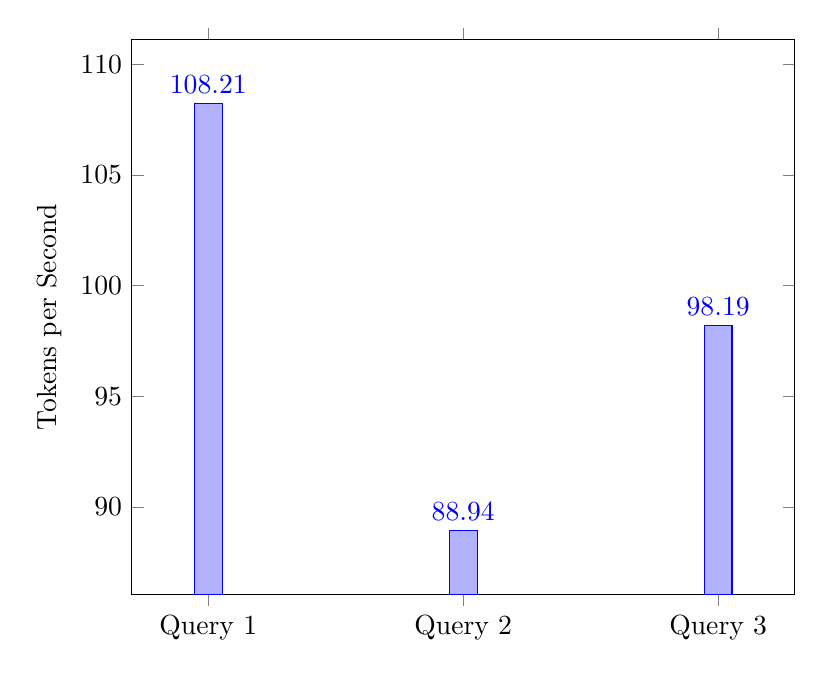
\begin{tikzpicture}
\begin{axis}[
    ybar,
    enlargelimits=0.15,
    legend style={at={(0.5,-0.15)},
      anchor=north,legend columns=-1},
    ylabel={Tokens per Second},
    symbolic x coords={Query 1, Query 2, Query 3},
    xtick=data,
    nodes near coords,
    nodes near coords align={vertical},
]
\addplot coordinates {(Query 1,108.21) (Query 2,88.94) (Query 3,98.19)};
\end{axis}
\end{tikzpicture}
\caption{Generation throughput (Tokens/Second) for three test queries.}
\label{fig:throughput}
\end{figure}

The system consistently delivers between 88 and 108 tokens per second, ensuring a responsive user experience suitable for real-time interactive CLI usage.

\section{Conclusion}

\texttt{ragcli} demonstrates that I have effectively implemented a modern RAG pipelines as a local CLI tool without sacrificing performance. By combining Oracle Database 23ai's robust vector search with the lightweight \texttt{gemma3:270m} model, I achieved sub-second retrieval times and generation speeds exceeding 90 tokens per second. Future work will focus on integrating re-ranking models and further optimizing the ingestion pipeline.

\end{document}
